% Explanation as Architecture — master document.
% Build: Overleaf (pdfLaTeX + shell-escape for the svg package), or
% locally with inkscape on PATH. See README.md in this directory.
\documentclass[sigplan,10pt,review]{acmart}

\usepackage{booktabs}
\usepackage{tikz}
\usetikzlibrary{arrows.meta,positioning,fit}
\usepackage{svg}      % F7 (requires shell-escape; Overleaf has it)
\usepackage{listings}

% Draft conveniences — removed at camera-ready.
\settopmatter{printfolios=true}

\lstset{basicstyle=\ttfamily\scriptsize, breaklines=true,
        frame=single, framesep=4pt, columns=fullflexible}

\begin{document}

\title{Explanation as Architecture: Recorded Traces, Provenance, and
Testable Diagnostics in Compiler Construction}

\author{Lojan Essam ElDin Farouk}
\email{lojanessamfarouk@gmail.com}
\affiliation{\institution{Independent}\country{}}

\begin{abstract}
Compilers routinely discard the evidence behind their own
diagnostics: the analysis knew which function it was checking, which
grammar rule it was inside, and which check failed, but what survives
to the user is a rendered string and a location. We present an
architecture that treats explanation as a first-class obligation of
every pipeline stage rather than a presentation-layer afterthought.
Every diagnostic is a structured artifact carrying a trace
\emph{recorded from the compiler's actual execution}; all explanatory
prose lives in a root-cause-indexed knowledge base isolated from the
stages; source provenance survives lowering and optimization into the
emitted assembly; and diagnostic-quality properties --- cascade-freedom,
trace accuracy --- are enforced as executable tests. We validate the
architecture in a complete, zero-dependency compiler for a C-like
kernel language ($\sim$5.9K LOC, 205 tests) and measure its costs
factorially: naive always-on trace recording cost $2.4\times$ compile
time and was repaired to statistical insignificance by lazy detail
formatting; provenance costs a steady 12--17\%, attributable to
per-instruction metadata growth (116$\to$160 bytes); peak memory is
unaffected. We report negative results as findings, including the
non-transitivity of per-instruction provenance under dead-code
elimination. The term ``explanation'' here denotes preserved compiler
evidence, not machine-learning explainability, and no claims about
human benefit are made without the user study we design but do not
run.
\end{abstract}

\maketitle

\section{Introduction --- draft v1}
\label{sec:intro}

During this compiler's development, its semantic analyzer detected a
program defect and told no one. The program was `int main() { int x
= 5; }` --- a non-void function that never returns. The analyzer's
internal log recorded the failure precisely ("bare return in
non-void function"); no diagnostic was ever constructed from that
knowledge; compilation "succeeded"; and the produced binary returned
whatever value happened to occupy the return register. The compiler
knew. The user didn't. We found the defect not by reading the code
but by running twenty adversarial programs against the finished
compiler --- and we report it as the paper's motivating observation
because it is the general phenomenon in miniature: **the evidence
behind compiler diagnostics is routinely discarded before, or
instead of, reaching the user.** What a conventional pipeline
retains at the point of failure --- a message string and a source
location --- is a small projection of what it knew moments earlier:
the construct being analyzed, the rule being applied, the path taken
to get there, and what became of the user's code in every stage
downstream.

This is not the familiar complaint that error messages are unhelpful.
Message \emph{quality} has received sustained attention in production
compilers --- Rust's structured suggestions \cite{rust-rfc1644}, GHC's migration to
errors-as-values \cite{ghc-structured-errors} [$\rightarrow$\S5] --- and a substantial research literature
examines message effectiveness, with notably contested results:
controlled studies of \emph{enhanced} messages report effects ranging
from ineffectual to inconclusive \cite{denny2014enhancing,pettit2017enhanced}. We take that contestation seriously: this
paper makes no claim that its diagnostics help users more, and the
user study such a claim requires is designed but not run (\S13). Our
question is upstream of wording, and architectural: **what must a
compiler retain, and where must it retain it, for explanation to be
possible at all --- and what does retaining it cost?**

Two scope commitments frame everything that follows. First, the
vehicle is a deliberately small compiler: a C-like kernel language
(integers, arithmetic, functions without calls) compiled through a
complete pipeline --- lexing, recursive-descent parsing, semantic
analysis, three-address IR, three optimization passes run to a fixed
point, and 32-bit x86 code generation to a linked executable. The
contribution is the architecture and its measured costs, not a
production technique; scaling questions are discussed, not claimed
away (\S10). Second, "explanation" here means *preserved compiler
evidence* --- recorded execution paths, provenance, root causes --- not
post-hoc rationalization, and not machine-learning explainability.

The architecture rests on one obligation: no stage may discard the
evidence a future explanation would need. Concretely (Fig. F1 shows
one diagnostic carrying all of it): every stage returns its product
\emph{and} its diagnostics, so partial results survive errors; a
diagnostic is a structured value --- kind, severity, span, root cause,
explanation, fixes, examples, trace --- never a string; all prose
lives in one knowledge base indexed by root cause, so the taxonomy
is the explanation index; each stage owns a trace recorder whose
RAII scopes capture the \emph{actual} execution path, snapshotted at the
moment a diagnostic is created; every IR instruction carries its
source span and accumulates notes from the optimizer passes that
transform it, surfacing as source-line comments in the emitted
assembly; and the properties that make diagnostics trustworthy ---
one mistake yields one diagnostic; traces contain runtime facts ---
are regression tests, not aspirations.

Making that architecture honest required measuring it, and the
measurements pushed back. Our first overhead campaign measured the
harness, not the compiler, and was discarded (\S9.2 explains how, so
readers do not repeat it). The second refuted our own hypothesis:
naive trace recording --- eagerly building detail strings at every
scope entry --- cost 2.4$\times$ compile time at 20k lines, dominated by two
scopes per token in the lexer. The repair (lazy detail formatting
over caller-owned data, exploiting the fact that snapshots occur
only while frames are open) brought recording to 1--2\% with
confidence intervals spanning zero, with byte-identical output.
Provenance, by contrast, is \emph{not} free: a steady 12--17\%, mechanical
in origin --- the span and note fields grow every IR instruction from
116 to 160 bytes, and every copy and traversal pays. We also report
what provenance cannot promise: per-instruction history is not
transitive under dead-code elimination (a folded instruction's
history dies with it once propagation makes it dead), and our
cascade-freedom invariants, while holding on every tested shape,
leave a measured residual --- 3\% of single-fault mutants still
produce three or more diagnostics.

This paper contributes:

\begin{itemize}
\item \textbf{C1 --- an architectural pattern for explanation-oriented compilation:} the five-role diagnostic core (root-cause taxonomy, factory, isolated knowledge base, multi-target rendering) over a pipeline-wide output-plus-diagnostics contract --- presented as the distilled, designed-in form of a structure production compilers (GHC, Rust) have been converging toward by retrofit \cite{rust-rfc1644,ghc-structured-errors} [$\rightarrow$\S5].
\item \textbf{C2 --- execution-recorded diagnostic traces:} RAII scope recording with snapshot-at-creation and a curated fallback that is provably unreachable in the pipeline; with the lazy-formatting design that makes always-on recording statistically free, and the measurements for both designs.
\item \textbf{C3 --- end-to-end provenance under the same contract:} source spans and transformation notes surviving to emitted assembly --- conceding LLVM's optimization remarks \cite{llvm-remarks} as production-scale prior art for the mechanism, and contributing its unification with the diagnostic architecture, its measured price, and the DCE non-transitivity finding.
\item \textbf{C4 --- diagnostic quality as executable invariants:} property- level tests (cascade-freedom, trace accuracy) distinct from golden-output snapshots, with mutation testing quantifying the frontier they do not yet cover.
\end{itemize}

\S4 fixes vocabulary and the language; \S5 positions against five
literature clusters; \S6 presents the architecture as fourteen
design decisions, each argued against a rejected alternative; \S7
describes the visualization consumer; \S8 the implementation; \S9 the
three-iteration measurement campaign and quality studies; Sections~10--13
discuss scaling, validity, limitations, and future work, including
the designed user study; \S14 concludes.




% Figures F1-F7. F1/F4/F5 are deliberately textual (they reproduce
% real compiler output / real IR states verbatim -- fact-ledgered in
% paper/figures/); F2/F3 are TikZ from the ledgered sources; F6 is a
% placeholder pending the capture protocol; F7 is the generated,
% self-checking SVG (tools/plot_overhead.py).

\begin{figure*}[t]
\begin{lstlisting}
ERROR TYPE:                          |  HOW TO FIX:
Malformed Expression                 |  Insert an operator between x and 2
                                     |  or remove the extra value
LOCATION:                            |
line 3, column 14                    |  TRACE:
    3 |     return x 2;              |  Parser
      |              ^               |  -> Parser::parse()
                                     |  -> Parser::parseFunctionDecl()
ROOT CAUSE:                          |       [starting at line 1]
Two expressions appeared             |  -> Parser::parseBlock()
consecutively with no operator       |  -> Parser::parseStatement()
between them.                        |       [at 'return' (line 3)]
                                     |  -> Parser::parseReturnStmt()
WHAT HAPPENED:                       |       [at 'return' (line 3)]
The parser successfully read:        |  -> DiagnosticEngine::
    return x                         |       malformedExpression()
After completing that expression,    |       [diagnostic created]
it encountered another value:        |
    2                                |  INVALID:   x 2
C++ requires an operator             |  VALID:     x + 2
between values.                      |             x * 2
                                     |             x = 2
\end{lstlisting}
\caption{One diagnostic, verbatim (two-column arrangement of the
CLI's sequential output). Every field is data on one struct
(\S\ref{sec:architecture}): the trace is recorded from the parser's
actual descent with runtime details in brackets, the examples are
synthesized from the offending tokens, and the same value renders
identically in the visualizer (Fig.~\ref{fig:f6}).}
\label{fig:f1}
\end{figure*}

\begin{figure}[t]
\centering
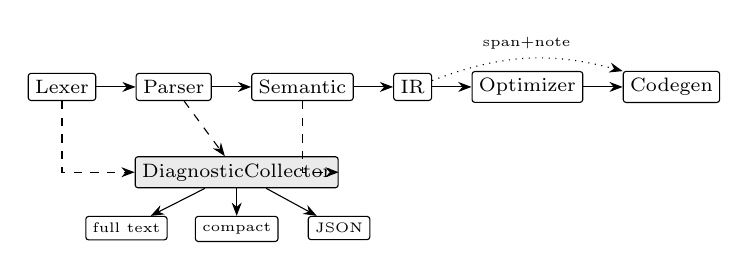
\begin{tikzpicture}[node distance=3.5mm and 5mm, >={Stealth},
  st/.style={draw, rounded corners=1pt, font=\scriptsize, inner sep=2.5pt},
  dg/.style={draw, rounded corners=1pt, font=\scriptsize, inner sep=2.5pt, fill=black!8},
  e/.style={->, font=\tiny}]
\node[st] (lx) {Lexer};
\node[st, right=of lx] (ps) {Parser};
\node[st, right=of ps] (sa) {Semantic};
\node[st, right=of sa] (ir) {IR};
\node[st, right=of ir] (op) {Optimizer};
\node[st, right=of op] (cg) {Codegen};
\node[dg, below=7mm of ps, xshift=8mm] (dc) {DiagnosticCollector};
\node[st, below=3.5mm of dc, xshift=-14mm] (r1) {\tiny full text};
\node[st, below=3.5mm of dc] (r2) {\tiny compact};
\node[st, below=3.5mm of dc, xshift=13mm] (r3) {\tiny JSON};
\draw[e] (lx) -- (ps); \draw[e] (ps) -- (sa); \draw[e] (sa) -- (ir);
\draw[e] (ir) -- (op); \draw[e] (op) -- (cg);
\draw[e, dashed] (lx) |- (dc);
\draw[e, dashed] (ps) -- (dc);
\draw[e, dashed] (sa) |- (dc);
\draw[e] (dc) -- (r1); \draw[e] (dc) -- (r2); \draw[e] (dc) -- (r3);
\draw[e, dotted] (ir) to[bend left=18] node[above, font=\tiny]{span+note} (cg);
\end{tikzpicture}
\caption{The pipeline with its diagnostics spine. Every front-end
stage returns output \emph{and} diagnostics (D1); IR, optimizer, and
codegen emit none by design (D2) --- but carry provenance (dotted).
Three renderers consume one struct (D6).}
\label{fig:f2}
\end{figure}

\begin{figure}[t]
\centering
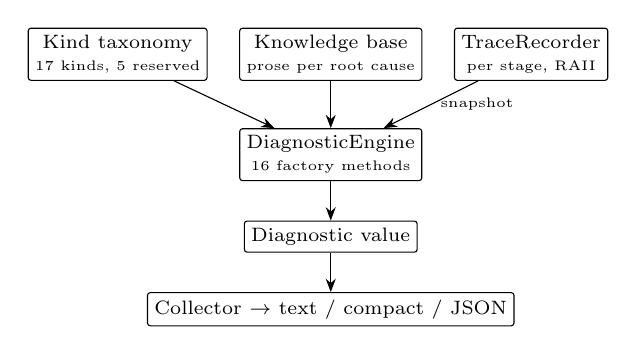
\begin{tikzpicture}[node distance=3mm and 4mm, >={Stealth},
  r/.style={draw, rounded corners=1pt, font=\scriptsize, align=center, inner sep=2.5pt},
  e/.style={->, font=\tiny}]
\node[r] (k) {Kind taxonomy\\ \tiny 17 kinds, 5 reserved};
\node[r, right=of k] (kb) {Knowledge base\\ \tiny prose per root cause};
\node[r, right=of kb] (tr) {TraceRecorder\\ \tiny per stage, RAII};
\node[r, below=6mm of kb] (en) {DiagnosticEngine\\ \tiny 16 factory methods};
\node[r, below=5mm of en] (d) {Diagnostic value};
\node[r, below=5mm of d] (c) {Collector $\to$ text / compact / JSON};
\draw[e] (k) -- (en); \draw[e] (kb) -- (en);
\draw[e] (tr) -- node[right, font=\tiny]{snapshot} (en);
\draw[e] (en) -- (d); \draw[e] (d) -- (c);
\end{tikzpicture}
\caption{The five-role diagnostic core (\S\ref{sec:architecture});
the fifth role, the \texttt{StageOutput} transport, is Fig.~\ref{fig:f2}'s
spine. The knowledge-base edge also carries the curated fallback
chains, unreachable in the pipeline (D8).}
\label{fig:f3}
\end{figure}

% F4 is folded into F1's trace panel for space at first assembly; a
% dedicated sequence diagram is cut unless a reviewer asks. The
% ledgered source remains in paper/figures/F2-F5-diagram-sources.md.

\begin{figure}[t]
\begin{lstlisting}
source (line 2):   return (2 + 3) * 4;

before        iteration 1          iteration 2         final
[2] t0 = 2+3  CF: t0 = 5           (t0 gone)
                 ;folded from
                  't0 = 2 + 3'
[2] t1 = t0*4 CP: t1 = 5 * 4       CF: t1 = 20         (t1 gone -- its
                 ;t0->5 (CopyProp)    ;t0->5; folded     fold AND prop
              DCE: t0 removed          from 't1 = 5*4'   notes die)
                  (fold note dies) CP: return 20
[2] return t1     return t1           ;t1->20 (CopyProp)
                                   DCE: t1 removed     [2] return 20
                                                          ;t1->20 (CopyProp)
\end{lstlisting}
\caption{Provenance through the fixed point for \texttt{(2+3)*4}.
The source line survives every rewrite; transformation notes
accumulate --- and die twice with the instructions DCE removes. The
single surviving instruction reports only the propagation step:
per-instruction provenance is honest but not transitive
(\S\ref{sec:limitations}, item 3).}
\label{fig:f5}
\end{figure}

\begin{figure}[t]
\centering
\fbox{\parbox{0.9\linewidth}{\centering\scriptsize\vspace{8mm}
F6: visualizer screenshot --- capture per
\texttt{paper/figures/F6-F7-notes.md} (full-config build; same
program family as Fig.~\ref{fig:f1}).\vspace{8mm}}}
\caption{The visualizer rendering the same diagnostic value as
Fig.~\ref{fig:f1}: identical sections, identical recorded trace,
because both surfaces are renderers over one struct (D6). Right: IR
panel with per-instruction source-line gutters and optimizer notes.}
\label{fig:f6}
\end{figure}

\begin{figure*}[t]
\centering
\includesvg[width=0.95\textwidth]{figures/F7-overhead}
\caption{Always-on overhead of the explanation architecture versus
the ablated baseline, before and after the lazy-formatting repair
(D14), across program sizes (log scale). Whiskers: 95\% bootstrap
CIs. Left: eager detail strings cost up to $\sim$175\% (trace) and
$\sim$160\% (full). Right, same scale: recording collapses to CIs
spanning zero; the remaining 12--17\% is provenance
(\S\ref{sec:eval}). Generated by a script that hard-asserts every
plotted median against the paper's tables.}
\label{fig:f7}
\end{figure*}

\section{Background --- draft v1}
\label{sec:background}

\subsection{Vocabulary}

Four terms carry precise meanings in this paper. A \textbf{diagnostic} is
a structured value describing one user-source mistake: kind,
severity, source span, message, root cause, explanation, ordered
fixes, optional invalid/valid examples, and a trace. A \textbf{trace} is
the sequence of compiler activities that led to a diagnostic's
creation; this paper distinguishes \emph{recorded} traces (snapshots of
the frames actually open at creation time) from \emph{curated} ones
(hand-written reference chains --- the fallback, \S6.3). \textbf{Provenance}
is the backward link from a compiled artifact to its origin: which
source line an IR instruction or assembly block derives from, and
which optimization decisions transformed it. \textbf{Explanation} is the
umbrella for all of the above --- preserved compiler evidence, not
machine-learning explainability and not post-hoc rationalization.

\subsection{The source language}

The vehicle is a C-like kernel language --- deliberately not "a C++
subset" in any meaningful sense, though its programs are valid C.
The complete grammar (verbatim from the parser's specification
comment):

\begin{verbatim}
program       -> function_decl*  EOF
function_decl -> type IDENT '(' param_list ')' block
param_list    -> (type IDENT (',' type IDENT)*)  |  (empty)
block         -> '{' statement* '}'
statement     -> var_decl | return_stmt
var_decl      -> type IDENT ('=' expression)? ';'
return_stmt   -> 'return' expression? ';'
expression    -> assignment
assignment    -> IDENTIFIER '=' assignment | equality
equality      -> comparison (('=='|'!=') comparison)*
comparison    -> addition   (('<'|'>') addition)*
addition      -> multiply   (('+'|'-') multiply)*
multiply      -> unary      (('*'|'/') unary)*
unary         -> primary
primary       -> INTEGER_LITERAL | IDENTIFIER | '(' expression ')'
type          -> 'int'
\end{verbatim}

Table T1 (feature inventory): \textbf{supported} --- \texttt{int} variables with
optional initializers; arithmetic and comparison operators with C
precedence; assignment as a right-associative expression
(\texttt{a = b = c}); multi-parameter functions; multi-error reporting with
panic-mode recovery. \textbf{Absent by design} --- control flow, function
calls, strings, arrays, pointers, unary operators, additional types.
Internally the type lattice contains \texttt{int}/\texttt{bool}/\texttt{unknown} (\texttt{bool}
arises only as a comparison result; \texttt{unknown} is the error-recovery
type that suppresses cascading type errors) and \texttt{void} (reserved).

The smallness is the method, not a concession: every architectural
mechanism must be visible whole, every diagnostic kind enumerable
(seventeen, of which five are explicitly reserved-unreachable), and
every claim checkable against a codebase a reviewer can actually
read (\textasciitilde{}5.9K lines, \S8).

\subsection{The pipeline}

Compilation proceeds through eight stages: lexing (single-pass,
maximal-munch), recursive-descent parsing to an AST whose nodes are
pure data traversed by four independent visitors, semantic analysis
(scope-stack symbol table; type resolution annotating the AST),
lowering to a flat three-address IR, three optimization passes
(constant folding, copy propagation, dead-code elimination) run
together to a fixed point, code generation to 32-bit x86 assembly
text, and an OS-facing driver that assembles and links a real
executable via the system toolchain. The construction follows
standard practice throughout \cite{aho2006compilers}; nothing in the
pipeline itself is claimed as a contribution. What \S6 adds is the
explanation obligation threaded through every one of these stages ---
and \S9 the bill for it.




\section{Related Work --- draft v1}
\label{sec:related}

Five clusters position this work; the two concessions come first,
because a reviewer should meet them in our words before theirs.

\subsection{Structured diagnostics in production compilers}

Production compilers have been converging on diagnostics-as-data by
retrofit. Rust formalized its error format and structured
suggestions in RFC 1644 \cite{rust-rfc1644}, emits machine-consumable JSON
diagnostics \cite{rustc-json}, and maintains Fluent-based message infrastructure
with a public error index \cite{rustc-dev-guide}. GHC's migration from \texttt{SDoc} strings
to "errors as structured values" --- with \texttt{diagnosticReason} and
\texttt{diagnosticHints} fields and public error codes since 9.6.1 --- is
documented across its development tracker and implementers' reports
\cite{ghc-structured-errors,welltyped2021ghc}, and the community maintains an error index \cite{haskell-error-index}. **Concession
one:** the five-role core of \S6.2 is therefore not a new invention
but a distillation; our claims are that designing it in from the
first commit is cheap (\S8), that the isolated knowledge base and
root-cause-granularity taxonomy are the load-bearing choices (\S6,
D3--D4), and that the retrofit pain documented by these projects [4,
9] is evidence the pattern matters. To our knowledge, none of these systems
provides the recorded per-diagnostic execution trace of \S6.3. That
knowledge is not passive: a targeted counterexample sweep (recorded
in the reference registry) found only adjacent work --- trace tooling
for \emph{student programs} \cite{suzuki2017tracediff}, and compiler-internal debug dumps
aimed at the compiler's own developers rather than its users --- and
if later work surfaces, this sentence and C2 narrow accordingly.

\subsection{Optimization transparency and provenance}

LLVM's remarks infrastructure \cite{llvm-remarks} is production-scale prior art for
per-transformation records: passes emit typed remark objects with
source locations, serialized to YAML and visualized with dedicated
tools. \textbf{Concession two:} our per-instruction notes are the same
mechanism at teaching scale. The residue we claim: unification of
provenance with the \emph{diagnostic} architecture under one contract
(one struct family, one renderer discipline, one JSON export), its
measured always-on price (12--17\%, \S9.2 --- LLVM's remarks are opt-in
per build), the human-readable in-text form (\texttt{\# line N:} comments in
the emitted assembly, by analogy to \texttt{.loc} directives but for
readers), and the negative result that per-instruction history is
not transitive under dead-code elimination (\S6.4, \S9).

\subsection{Error-message quality and its contested effectiveness}

A half-century of work examines programming error messages; Becker
et al.'s working-group report maps the landscape \cite{becker2019unhelpful}. Eye-tracking
evidence shows developers genuinely read error messages and that
reading difficulty predicts task performance \cite{barik2017developers}; design guidance
for novice-facing messages continues to develop \cite{denny2021designing}. Yet controlled
studies of \emph{enhanced} messages report effects from ineffectual \cite{denny2014enhancing}
to inconclusive \cite{pettit2017enhanced} --- a contested record extending into the LLM era,
where generated explanations show promise in some deployments \cite{taylor2024dcc}
and ineffectiveness in others \cite{santos2024silver}. This contestation shapes our
claim discipline (\S9.3): we measure component \emph{presence} with a
mechanical instrument descended from Marceau et al.'s evaluation
rubric \cite{marceau2011measuring}, and defer all helpfulness claims to a designed-but-
unexecuted study (\S13). Our contribution is orthogonal to wording
quality: an architecture that \emph{retains the evidence} any wording ---
human-authored or LLM-generated \cite{taylor2024dcc} --- would need.

\subsection{Error localization and interrogative debugging}

Constraint-based localization computes \emph{where} the likely mistake
is: general static-error diagnosis via Bayesian-ranked unsatisfiable
constraints \cite{zhang2014general,zhang2017sherrloc}, type-error diagnosis \cite{zhang2015diagnosing}, and SMT-based
localization \cite{pavlinovic2015smt}. These are complementary: they improve one field
of our diagnostic (the span and root-cause selection), while our
architecture governs how the whole explanation is assembled,
preserved, and delivered. The Whyline \cite{ko2008debugging,ko2010extracting} pioneered
why/why-not questions over \emph{program} executions via tracing and
slicing, a family that extends into education through trace-
divergence debugging of student code \cite{suzuki2017tracediff}; we ask the interrogative
question of the \emph{compiler's own run} --- a far shallower trace,
recorded live at negligible cost (\S9.2) rather than reconstructed by
post-hoc analysis.

\subsection{Compiler visualization in education}

The lineage is old --- the UW Illustrated Compiler graphically
displayed its own control and data structures to students in 1988
\cite{andrews1988uw} --- and continues through AST construction animators \cite{almeida2008vast},
interactive stage simulations \cite{rodriguez2013simulations}, and, recently, JIT IR-evolution
explorers \cite{dalbo2025jitscope}. Our visualizer (\S7)
sits in this lineage as a \emph{consumer} of the architecture rather than
a contribution: its distinguishing property is that every panel
renders the same structured values the CLI renders, because the
architecture guarantees a single source of truth (\S6.2, D6).

\subsection{Positioning summary (Table T2)}

\begin{table}[t]
\centering
\small
\begin{tabular}{lllll}
\toprule
Capability & GHC \cite{ghc-structured-errors} & rustc \cite{rust-rfc1644,rustc-dev-guide,rustc-json} & LLVM \cite{llvm-remarks} & this work \\
\midrule
Structured diagnostics as values & retrofit & retrofit & --- & designed-in \\
Root-cause-indexed public error index & \checkmark{} \cite{haskell-error-index} & \checkmark{} & --- & \checkmark{} (taxonomy = index, D3) \\
Machine-readable diagnostic export & \checkmark{} & \checkmark{} \cite{rustc-json} & \checkmark{} (remarks) & \checkmark{} \\
Per-diagnostic \textbf{recorded execution trace} & --- & --- & --- & \checkmark{} (\S6.3) \\
Optimization provenance records & --- & --- & \checkmark{} opt-in \cite{llvm-remarks} & \checkmark{} always-on, unified, priced \\
Diagnostic-quality \textbf{property} tests & snapshot-style & golden \texttt{.stderr} \cite{rustc-dev-guide} & --- & property-level + mutation-measured (\S9) \\
\bottomrule
\end{tabular}
\end{table}




\section{The Explanation Architecture --- draft v2.1}
\label{sec:architecture}



The architecture rests on a single obligation: *no stage may discard
the evidence a future explanation would need*. This section presents
the four mechanism groups that discharge that obligation --- the stage
contract (\S6.1), the diagnostic core (\S6.2), recorded traces (\S6.3),
and cross-stage provenance (\S6.4) --- each as an engineering decision
weighed against at least one rejected alternative.

\subsection{Stage contract and the taxonomy of failure}

Every pipeline stage returns \texttt{StageOutput<T>}: its product \emph{and} a
list of structured diagnostics, always both. A stage that finds
errors still returns its partial product; the driver, not the stage,
decides whether to continue.

\textbf{D1 --- Partial-success contract vs. fail-fast propagation.} The
conventional alternatives are exceptions or an \texttt{Either}-style
short-circuit (\texttt{Result<T,E>} end to end). We rejected both for the
\emph{pipeline} path because explanation quality depends on surviving the
first error: a fail-fast parser cannot report the second, independent
mistake, and --- more damaging for this architecture --- it discards the
partially built AST that later explanation surfaces (the visualizer
deliberately renders the recovered-but-erroneous tree, because
\emph{where the parser got confused} is itself explanatory). The cost of
the choice is real: every stage must define what "partial product"
means (the parser synthesizes placeholder nodes; the analyzer types
what it can and poisons the rest with \texttt{unknown}), and downstream code
must tolerate it. Production compilers pay the same cost for the same
reason --- multi-error reporting has been standard since panic-mode
recovery; see \cite{diekmann2020dont} for the modern treatment and its quantified
failure mode, cascading. Evidence: \texttt{StageOutput<T>} in
\texttt{src/diagnostics/Diagnostic.hpp}; the parser's recovery paths and the
cascade-freedom tests they carry.

\textbf{D2 --- Three failure currencies vs. one.} A uniform "everything is
a \texttt{Diagnostic}" design was rejected because it conflates three
audiences. User-source mistakes become \texttt{Diagnostic} (they have a
\texttt{SourceSpan}; there is something to explain). Environment failures ---
assembler missing, disk full --- become \texttt{Result<T,E>}
(\texttt{src/driver/Toolchain.cpp}): they have no span, and routing them
through the explanation machinery would manufacture explanations for
facts about the machine, not the program. Violated *compiler
invariants* are \texttt{assert}s (\texttt{src/ir/IRGenerator.cpp}): a bug in us,
not in the user, and dressing it as a user-facing diagnostic would be
a category error with a friendly font. The cost: three idioms to
learn, and the boundary must be policed in review. The split mirrors
LLVM's separation of recoverable errors ("an error in the program's
environment... a missing file", handled via \texttt{Expected<T>}/\texttt{Error})
from its diagnostic subsystem \cite{llvm-programmers-manual}. Our own history enforces the boundary's
value: the one failure that \emph{was} misfiled (missing-return, logged
internally as neither diagnostic nor error) produced the
silent-garbage defect that motivates \S3.

\subsection{The five-role diagnostic core}

A diagnostic here is one struct carrying kind, severity, span,
message, root cause, explanation, ordered fixes, trace, and optional
invalid/valid example pairs. Five roles cooperate to build and
deliver it: a \textbf{kind taxonomy}, a \textbf{factory} (\texttt{DiagnosticEngine}),
a \textbf{knowledge base} (\texttt{ExplanationBuilder}), a \textbf{collector} with
three renderers, and the stage contract of \S6.1 as transport.

\textbf{D3 --- One kind per root cause vs. one code per message.}
\texttt{DiagnosticKind} allocates an enumerator per *distinct underlying
cause*, not per output string --- \texttt{PARSE\_MalformedExpression} covers
both \texttt{return x 2;} and \texttt{int x = 5 5;} because the mistake (two
expressions, no operator) is one cause with two surface forms. The
granularity rule is operational, not aesthetic: two failures share a
kind \textbf{iff} they share a root-cause sentence and a fix set --- the
knowledge base's own index structure decides. By contrast, a bare
\texttt{return;} in a non-void function and a \emph{missing} return entirely get
distinct kinds (\texttt{SEM\_ReturnTypeMismatch}, \texttt{SEM\_MissingReturn})
despite superficial kinship, because their causes, severities, and
fixes all differ --- one is an ill-formed statement (error), the other
a missing obligation (warning, GCC's \texttt{-Wreturn-type} choice). The
rejected alternative, message-granularity codes, is the shape
string-based systems drift into; GHC's and Rust's retrofits both
converged on cause-indexed identifiers with public indexes
\cite{haskell-error-index,ghc-structured-errors,rust-rfc1644}. Benefit: the
taxonomy \emph{is} the explanation index. Cost, honestly carried in the
header: taxonomy discipline requires admitting unreachable entries;
five kinds are marked \texttt{[reserved]} in
\texttt{src/diagnostics/DiagnosticKind.hpp} because the language cannot yet
produce them, and tests are forbidden from expecting them.

**D4 --- Centralized prose knowledge base vs. prose at the emit site
vs. external message DSL.** All user-facing explanation text lives in
one component, \texttt{ExplanationBuilder}, switch-indexed by kind and
parameterized by runtime detail. Emit-site prose (each stage writes
its own sentences) was rejected because it makes consistency
unenforceable and translation impossible --- the exact pathology GHC
documents in its \texttt{SDoc}-era retrofit discussion \cite{welltyped2021ghc,ghc-structured-errors}. The heavier
alternative --- an external message DSL (Clang's TableGen \texttt{.td} files
\cite{clang-internals}; rustc's Fluent \cite{rustc-dev-guide}) --- was rejected *at this
scale*: it buys tooling and i18n at the price of a build step
and an indirection layer, for seventeen kinds. The cost of our middle
position surfaced measurably: the builder's \texttt{detail}/\texttt{detail2}
interface hit its capacity limit the first time a kind needed three
context values, and the factory works around it by re-deriving one
field (\texttt{src/diagnostics/DiagnosticEngine.cpp}, documented at the
\texttt{malformedExpression} site). We report that as evidence about where
this design stops scaling; the industrial DSLs sit exactly where our
workaround points (see Discussion, \S10).

\textbf{D5 --- Factory/knowledge-base split vs. a merged emitter.}
\texttt{DiagnosticEngine} (runtime context in, complete struct out) is
separate from \texttt{ExplanationBuilder} (static text per kind). A merged
component would be smaller; the split was chosen because the two
change for different reasons --- one when \emph{detection} context changes,
one when \emph{wording} changes --- and because the knowledge base must stay
stateless and stage-independent for the fallback semantics of \S6.3 to
be sound. Cost: one more hop to read, and a factory method per kind
(mechanical boilerplate; sixteen methods at the time of writing).

\textbf{D6 --- Late rendering, three renderers vs. render-at-creation.}
Diagnostics are stored as data and rendered on demand --- full
explanatory text, compact one-liners, or JSON --- from the same struct
(\texttt{src/diagnostics/DiagnosticCollector.cpp}). Rendering at creation
(the string-concatenation norm this paper argues against) was
rejected as the root discard-point: once prose, always prose. The
measured consequence of late rendering is that CLI and visualizer
provably tell one story (they consume the same struct; Fig. F6), and
machine consumers get fields, not regexes --- the property GHC's and
Rust's JSON emitters retrofitted at cost \cite{rustc-json,ghc-structured-errors}. Cost: the struct is the compatibility surface;
adding a field touches all three renderers (the trace \texttt{detail}
field's addition did exactly that, in one commit).

\subsection{Recorded traces}

Every diagnostic carries the call path that produced it. The claim
requiring defense is the word \emph{recorded}.

**D7 --- RAII scope-stack snapshot vs. curated per-kind chains vs.
full event log.** The predecessor design --- and this is committed
history, not a rhetorical foil --- was a \emph{curated} chain: a
hand-written, plausible call path per kind, stored in the knowledge
base. It rendered convincingly and was architecturally cheap, but it
could not name the function being analyzed or the token under the
cursor, because those exist only at runtime; the paper's thesis calls
this fabricated provenance. The replacement: each stage owns a
\texttt{TraceRecorder}; methods at decision points open RAII scopes carrying
runtime detail ("function 'main'", "at 'return' (line 3)"); when the
factory builds a diagnostic it snapshots the frames \emph{currently open}
(\texttt{src/diagnostics/TraceRecorder.hpp}; Fig. F4 traces the sequence
for the Fig. F1 diagnostic). The third option --- logging
every event, not just the live stack --- was rejected on cost and noise
grounds: an event log grows with program size whether or not an error
ever occurs, while the active-stack snapshot is O(depth) and paid
only at diagnostic creation; the Whyline demonstrates the power of
full traces for \emph{program} debugging and also their price, a dedicated
post-hoc analysis apparatus \cite{ko2008debugging}. Disclosed cost
of our choice: sibling context is invisible (completed frames are
gone from the stack). The entry cost of open frames is the subject of
D14 and \S9.2 --- the naive version of this design failed its own
overhead experiment. Evidence that recording is real rather than
curated-with-extra-steps: a pre-existing regression test \emph{failed} at
the transition --- it had encoded the curated chain's shape
(\texttt{trace.front()} = detecting method), and recorded traces begin at
the true outermost frame instead. The failure was the proof; the test
now asserts containment.

\textbf{D8 --- Retaining the curated chains as fallback vs. deleting them.}
When an engine is used with no recorder attached --- unit tests
construct diagnostics directly --- the knowledge base's static chain is
substituted, and its final step (the factory method) is appended to
\emph{recorded} chains too, so every trace terminates identically.
Deleting the curated chains would have simplified the truth story at
the cost of either dragging recorder setup into every unit test or
letting traces go empty off-pipeline. We kept the fallback and
disclose it. In the compiled pipeline the fallback is unreachable:
exactly three \texttt{DiagnosticEngine} instances exist (one per
diagnostic-emitting stage), and each attaches its recorder before
parsing/analysis begins; IR generation, optimization, and code
generation emit no diagnostics at all. Every diagnostic a user can
ever see therefore carries a recorded trace (verified by exhaustive
search for engine instantiations). The residual risk we accept is
dual-source drift, mitigated by the shared final step and by tests
that assert \emph{recorded} traces contain runtime facts no static chain
could hold.

\textbf{D9 --- Selective scope placement vs. instrument-everything.}
Placement follows a stated rule, not taste: a scope is opened (i) in
every method that can itself emit a diagnostic, and (ii) at
structural landmarks that name the enclosing construct (function,
block, statement dispatch). Expression-precedence internals satisfy
neither --- their failures surface in \texttt{parsePrimary}/\texttt{expect}, which
are covered by (i). A skeptic may object that selective scoping makes
the recorded trace "curated by another name" --- the author still
chooses what is recordable. The objection conflates two different
failure modes. A curated chain can be \emph{wrong}: it asserts a path that
did not execute (and before this transition, ours did --- no curated
chain could have named \texttt{function 'main'}). A selectively scoped
recording can only be \emph{coarse}: every frame it reports was genuinely
open, verified by tests asserting runtime facts in the output.
Omission bounds resolution; it cannot manufacture provenance. The
placement policy is itself inspectable data (grep \texttt{TRACE\_SCOPE}), and
refining it is a local edit, not an architectural change.

\textbf{D13 --- Ablation by macro vs. no-op class (measurement honesty).}
The overhead experiments compare builds with recording compiled out.
A no-op \texttt{TraceScope} class would still evaluate its argument
expressions --- the detail context built at every call site --- and so
would silently understate the mechanism's true cost. Call sites
therefore use a \texttt{TRACE\_SCOPE(...)} macro that erases its arguments
entirely under \texttt{-DCPPC\_NO\_TRACE}. Cost: a macro where RAII would be
idiomatic; accepted because a measurement that flatters the design is
worse than an ugly line. (The same flag design gives the factorial
attribution used in \S9.2.)

**D14 --- Lazy detail formatting vs. eager strings (added after E1
refuted H3 for the eager design).** The first recorder built each
frame's detail \emph{string} at scope entry. E1 measured that at \textasciitilde{}2.4$\times$
total compile time on 20k-line inputs --- the lexer opens two scopes
per token, so a clean compile paid for hundreds of thousands of
string constructions whose text nobody would ever read. The repaired
design stores lazily-formattable POD in each frame --- \texttt{const char*}
literals, a pointer to a caller-owned string, ints --- and materializes
text only in \texttt{snapshot()}, i.e. only when a diagnostic fires. Two
correctness arguments carry the design: (1) \emph{pointer stability} ---
snapshots only ever occur while frames are open (the engine runs
inside the stage method that owns the scope), so a frame may safely
point at a token's lexeme or an AST node's name, which provably
outlive it; rvalue overloads are deleted so a temporary cannot be
captured. (2) \emph{Entry-time semantics} --- ints (line/column) are copied
by value at scope entry because the lexer's counters advance during
the scope, and the frame must describe where the scope was \emph{opened},
exactly as the eager strings did. One rare path (the parser's
empty-lexeme case) needs text whose construction would couple the
diagnostics layer to the lexer; it pays for an eager string via an
explicit escape hatch rather than couple the layers. Alternatives
rejected: deferred closures (a \texttt{std::function} per frame allocates ---
the disease as the cure) and fixed-size \texttt{snprintf} buffers (kills the
allocation but keeps per-scope formatting work and truncates
unpredictably). The materialized strings are byte-identical to the
eager versions --- the trace-content tests pin them, and passed
unchanged across the transition. Measured effect (\S9.2, interleaved
protocol): recording cost fell from +143\% [130, 168] to 1--2\% with
confidence intervals spanning zero at every corpus size --- a \textasciitilde{}60$\times$
reduction, leaving recording statistically indistinguishable from
free while producing identical output.

\subsection{Provenance to emitted assembly}

**D10 --- Inline provenance fields vs. side tables vs. AST
back-pointers.** Every \texttt{IRInstruction} carries a \texttt{SourceSpan} and a
transformation \texttt{note} as ordinary value fields, stamped at lowering
(\texttt{src/ir/IRGenerator.cpp}). Back-pointers into the AST were rejected
on lifetime grounds --- they would couple IR validity to AST retention,
which no later consumer otherwise needs. A side table (instruction $\rightarrow$
span) was rejected on \emph{identity} grounds: optimizer passes rewrite
instructions in place and rebuild instruction vectors (DCE), so any
table keyed by identity or index desynchronizes precisely when
provenance matters most; inline fields travel with the value through
every rewrite for free. Constant folding's rewrite demonstrates the
discipline the choice demands (quoted from
\texttt{src/optimizer/ConstantFoldingPass.cpp}):

\begin{verbatim}
// Provenance: the replacement must keep the original's source span
// (it still comes from the same source expression) and record what
// it used to be -- rebuilding via makeCopy() alone would silently
// wipe both.
IRValue     dest   = instr.dest;
SourceSpan  span   = instr.span;
std::string before = instr.toString();
std::string prior  = instr.note;
instr = IRInstruction::makeCopy(dest, IRValue::makeConst(result));
instr.span = span;  instr.note = prior;
instr.appendNote("folded from '" + before + "' (ConstantFolding)");
\end{verbatim}

The four saved locals are the cost of inline provenance made visible:
every rewriting pass owes this discipline. A side table would trade
those four lines for an identity-tracking problem across in-place
rewrites and DCE's vector rebuild --- a worse debt, but a real
alternative for pass-heavy compilers. Costs of inline fields, both
measured (\S9.2): the enlarged instruction makes every copy, move,
and pass traversal pay --- a steady 12--17\% wall time --- while peak
memory stays $\leq$1.3\%; provenance's price is time, not space. And
\texttt{toString()} had to stay byte-stable so thirty golden IR tests
survived; provenance display therefore lives in separate channels
(structured JSON, assembly comments) rather than in the canonical
text.

\textbf{D11 --- Accumulated string notes vs. structured remark records.}
Passes append human-readable notes ("\texttt{t1 -> 20 (CopyPropagation)}").
The structured alternative is exactly what LLVM ships --- typed remark
objects serialized to YAML with dedicated viewers \cite{llvm-remarks} --- and we
concede it is the scalable form. Strings were chosen because at this scale the consumer
is a human reading a panel or a \texttt{.s} file, and a remark schema would
be structure nothing downstream parses. The choice exposed a genuine
finding the structured design would \emph{also} exhibit: per-instruction
history is \textbf{not transitive}. When DCE removes a folded instruction
whose constant was already propagated onward, its ConstantFolding
note dies with it; the surviving instruction reports only the
propagation step (Fig. F5 walks the fixed-point iterations for
\texttt{(2+3)*4}). Both the optimizer and visualizer suites lock this
behavior in as documented semantics rather than accident --- and it
delimits what per-instruction provenance can ever promise without a
dataflow-chained design (Future Work, \S13).

**D12 --- Comment-based assembly provenance vs. debug-info
directives.** Codegen emits \texttt{\# line N: <ir> ; <notes>} above each
instruction block. The rejected alternative --- \texttt{.loc}/DWARF --- is the
production answer and is \emph{machine}-consumable by debuggers; it was
rejected here because our consumer is a reader, our 2006-era target
toolchain makes DWARF plumbing a project of its own, and the paper's
claim is about preserving explanation, not shipping debuggers. Cost:
tools cannot consume our provenance from the binary; it lives in the
text artifacts (assembly comments, JSON) only.

---


\section{The Visualization Consumer --- draft v1}
\label{sec:visualizer}

The visualizer exists in this paper as *evidence about the
architecture*, not as a contribution in the visualization lineage it
belongs to --- a lineage reaching back to the UW Illustrated Compiler,
which displayed its own control and data structures to students in
1988 \cite{andrews1988uw} (\S5.5). Its claim is narrow: because explanation is
preserved as structured data (\S6), building a full-pipeline
inspection surface required no new information channels --- only
renderers.

One CLI mode (\texttt{--json}) emits the entire compilation as a single
JSON object: tokens with positions, the type-annotated AST, the
semantic check log, IR before and after optimization (both as
display text and as structured per-instruction records with source
line and transformation note), the optimization reports, the final
assembly text, and the diagnostics with their recorded traces. The
export has a fixed shape: a stage that never ran contributes an
explicit empty value, never an absent key, so consumers need no
existence logic. A stdlib-only local server shells out to the
compiled binary per request; the frontend is framework-free
JavaScript rendering one tab per stage (Fig. F6). Stages that did
not run say why ("no semantic checks ran --- lex/parse stopped
first"), which is itself explanation: the pipeline's control-flow
decisions are user-visible state.

Two properties matter for the thesis. First, **single source of
truth**: the diagnostics tab renders the same struct the CLI
renders --- same sections, same recorded trace with the same runtime
details, same invalid/valid examples --- because both are renderers
over one value (D6); divergence between the two surfaces was an
actual defect class earlier in this project's history, eliminated
by construction rather than by discipline. Second, **provenance
becomes navigable**: the IR panels carry per-instruction source-line
gutters and optimizer notes from the same fields codegen prints as
assembly comments, so "which line did this instruction come from,
and what happened to it" is answerable in every representation the
compiler has.

The design deliberately avoids claiming more: there is no
cross-panel linked highlighting (clicking an assembly line does not
select its source token), no time-travel through optimizer
iterations, and no user evaluation of the interface --- the first two
are engineering the exported data already supports (\S13), the third
is out of scope with the rest of the human questions (\S11).




\section{Implementation --- draft v1}
\label{sec:impl}

\subsection{Shape and size}

The reference compiler is \textasciitilde{}5,943 lines of C++14 (measured at session
B; re-measure at submission) with zero external dependencies --- the
test framework, JSON emission, and visualization server are
hand-rolled or stdlib-only, so the artifact builds from a compiler
and Make alone. Distribution by subsystem:

\begin{table}[t]
\centering
\small
\begin{tabular}{lllll}
\toprule
subsystem & LOC &  & subsystem & LOC \\
\midrule
diagnostics & 1,739 &  & ast (4 visitors) & 500 \\
parser & 695 &  & main/driver CLI & 499 \\
semantic & 604 &  & lexer & 421 \\
ir & 463 &  & codegen & 385 \\
optimizer & 370 &  & core + toolchain & 267 \\
\bottomrule
\end{tabular}
\end{table}

The headline number is the first row: **the diagnostics subsystem is
the largest in the compiler --- 29.3\% of the source** --- which is the
architecture's priority expressed as a measurement rather than a
slogan. (The share has grown across the project: 27\% at the initial
audit, 28.2\% after trace recording, 29.3\% after lazy formatting.)

\subsection{Mechanism invasiveness (E5)}

From the introducing commit's diff, compiler source only: trace
recording cost $\approx$200 lines (the recorder, three stage integrations,
and surfacing through the renderers), and provenance $\approx$115 lines (IR
fields, generator stamping, preservation discipline in two passes,
assembly comments, JSON export) --- $\approx$320 lines across 17 files, \textasciitilde{}5.6\%
of the then-current source, for both mechanisms. The lazy-formatting
repair (D14) later replaced the recorder's internals and touched the
20 scope call sites mechanically. H1's "localized mechanisms" claim
rests on these numbers, with the honest caveat that locality was
measured in a codebase designed to receive the mechanisms; \S10
discusses what retrofit would change.

\subsection{Testing as method}

205 tests across nine suites (603 assertions) enforce three
distinct kinds of claim. Unit suites pin stage behavior. End-to-end
suites refuse to mock: generated assembly is assembled and linked
with the real system toolchain, the produced executable is \emph{run},
and its process exit code is asserted --- if codegen is wrong, a real
binary misbehaves, not an abstraction. Property suites encode the
diagnostic-quality invariants of \S6 and \S9.4, including the
trace-accuracy tests whose runtime-fact assertions distinguish
recorded from curated traces, and the \texttt{--check} silence tests that
protect the measurement channel every number in \S9 depends on.
There is no CI and no coverage measurement --- stated as fact; the
suite runs on one platform, like everything else here.

\subsection{Empirical construction on a legacy target}

The target toolchain (GCC 6.3.0, MinGW.org, 32-bit) predates
reliable documentation for several of its contracts, so codegen
facts were established by probing rather than assumed: the CRT's
entry-point requirements (the \texttt{\_main} symbol and \texttt{call \_\_\_main}
sequence) were derived by diffing real \texttt{gcc -S} output on probe
files after link failures whose messages pointed nowhere near the
cause. The same empiricism extended to the measurement harness,
where three Windows process-management quirks (a null \texttt{ExitCode}
without a cached handle; peak-memory counters unreadable after
exit; \texttt{CreateProcess} rejecting relative forward-slash paths)
each produced data that \emph{looked} like compiler behavior until
reproduced in isolation --- the \S9.2 discarded-campaign note is the
largest instance of the same lesson. We record these because the
paper's numbers pass through this machinery, and a reader repeating
the experiments on Windows will meet the same artifacts.

\subsection{Availability}

The complete source, test suites, corpus generator, measurement and
analysis scripts, mutation tooling, raw result CSVs for every
campaign (including the discarded and superseded ones), and this
paper's working documents are in one public repository, tagged for
artifact evaluation at submission. Every number in \S9 regenerates
from three documented commands.




\section{Evaluation --- draft v1}
\label{sec:eval}



\subsection{Methodology}

We evaluate three measurable questions from \S3: the invasiveness of
the mechanisms (H1/E5), their always-on runtime and memory cost
(H3/E1/E2), and the structural-quality properties of the diagnostics
they enable (E3/E4). Human benefit is explicitly \emph{not} evaluated
(\S13 designs that study; \S11 explains why the claim is withheld).

\textbf{Workload.} Deterministic, seeded, \emph{valid} programs at 100 / 1,000
/ 5,000 / 20,000 lines (many 20--40-statement functions of mixed-depth
integer arithmetic). Valid programs are the fair worst case for this
architecture: every mechanism pays its cost and no diagnostic ever
redeems it.

\textbf{Measurement path.} \texttt{--check}: every stage through assembly text,
no JSON serialization, no toolchain subprocess, nothing printed on
success --- the stopwatch sees the compiler and only the compiler. This
mode exists because our first campaign timed \texttt{--json} and measured
the harness instead (\S9.2, "a discarded campaign").

\textbf{Design.} Factorial ablation over two compile-time flags
(recording, provenance), giving four binaries: FULL, NOTRACE,
NOPROV, BASELINE --- each mechanism's cost is attributed separately.
Ablation is by macro so argument expressions vanish too; a no-op
class would understate the cost it exists to measure (\S6.3, D13).

\textbf{Protocol.} Per (config, size): 3 warmups, 30 timed runs, 5
peak-working-set runs (sampled live; the counter is unreadable after
exit). Binaries built \texttt{-O2}. Statistics: median and MAD per cell ---
wall times on a desktop OS are right-skewed by scheduler and
antivirus interference, and medians resist those spikes; overhead is
(median\_config -- median\_baseline)/median\_baseline with a 95\%
bootstrap CI (10,000 resamples, percentile method, fixed seed).
Alternatives rejected: mean$\pm$SD assumes symmetry the data does not
have; comparing against production-compiler \emph{speed} would be
meaningless at this scale, so all comparisons are self-vs-self.

\textbf{Environment.} Intel Core i7-8665U @ 1.90 GHz, 32 GiB RAM,
Windows 11 Pro (build 26200), GCC 6.3.0 (MinGW.org, 32-bit target).
Single machine, single toolchain: an external-validity limit stated
in \S11, not an inconvenience to hide.

\subsection{Overhead (E1/E2)}

\textbf{A discarded campaign (methodological note).} Our first E1
collection timed \texttt{--json} with output piped through the measurement
shell. The numbers failed the coherence check we ran before accepting
any of them: ablated configurations measured \emph{slower} than the full
build, orderings flipped between sizes, and "baseline" was nine
seconds for a 20k-line file through an O(n) pipeline. The harness was
ingesting megabytes of serialized pipeline state per run --- we had
measured PowerShell. The dataset was deleted, the \texttt{--check} path
built, and the campaign rerun. We report this because measurement
pitfalls that are survived silently get repeated by readers.

**Naive recorder (eager detail strings) --- the result that refuted
H3.** Median $\pm$ MAD, ms:

\begin{table}[t]
\centering
\small
\begin{tabular}{lllll}
\toprule
lines & baseline & notrace & noprov & full \\
\midrule
100 & 46.9 $\pm$ 2.1 & 53.4 $\pm$ 2.5 & 58.3 $\pm$ 3.4 & 73.8 $\pm$ 4.1 \\
1,000 & 154.8 $\pm$ 14.9 & 188.7 $\pm$ 8.8 & 278.4 $\pm$ 5.2 & 335.6 $\pm$ 11.4 \\
5,000 & 570.9 $\pm$ 7.1 & 824.3 $\pm$ 48.3 & 1,569.9 $\pm$ 59.0 & 1,493.6 $\pm$ 53.5 \\
20,000 & 2,266.0 $\pm$ 133.0 & 2,237.9 $\pm$ 67.5 & 5,498.2 $\pm$ 312.7 & 5,824.2 $\pm$ 221.1 \\
\bottomrule
\end{tabular}
\end{table}

At 20,000 lines --- the startup-amortized row --- trace recording cost
+143\% [130, 168] (NOPROV) and the full configuration +157\%
[144, 204]. The cause is identifiable, not mysterious: the lexer
opens two scopes per token, each eagerly building detail strings ---
order 10$^5$--10$^6$ heap constructions per clean compile, all discarded.
This campaign also \emph{appeared} to show provenance as free (NOTRACE vs
BASELINE: --1.2\%, CI spanning zero) --- a reading the interleaved
protocol below corrects; under blocked measurement, whichever config
runs nearest the baseline in time inherits flattering drift.

\textbf{A second protocol iteration.} Re-measuring the lazy recorder under
the same blocked protocol produced medians that *decrease
monotonically in run order* across configs (1890 $\rightarrow$ 1813 $\rightarrow$ 1532 $\rightarrow$
1512 ms at 20k) --- the machine sped up as the campaign progressed, and
with mechanism costs now small, that drift dominated the
between-config deltas. The final protocol therefore interleaves
configs round-robin within each run index, rotating cycle order to
cancel position bias. Blocked data is archived, not used.

**Lazy recorder (D14), interleaved protocol --- the authoritative
table.** Fig. F7 plots both campaigns' overhead on one shared scale
(the flat right panel is the repair); the figure is generated from
the raw CSVs by a script that hard-asserts every plotted median
against the tables below, so figure and paper cannot silently
diverge. Median $\pm$ MAD, ms:

\begin{table}[t]
\centering
\small
\begin{tabular}{lllll}
\toprule
lines & baseline & notrace & noprov & full \\
\midrule
100 & 24.1 $\pm$ 0.9 & 27.0 $\pm$ 1.9 & 24.4 $\pm$ 1.0 & 25.8 $\pm$ 0.8 \\
1,000 & 78.6 $\pm$ 2.5 & 89.9 $\pm$ 2.6 & 79.9 $\pm$ 2.8 & 90.3 $\pm$ 2.5 \\
5,000 & 398.4 $\pm$ 12.1 & 467.2 $\pm$ 11.0 & 402.7 $\pm$ 12.1 & 467.8 $\pm$ 10.2 \\
20,000 & 1,549.5 $\pm$ 76.1 & 1,801.6 $\pm$ 76.5 & 1,585.8 $\pm$ 94.7 & 1,844.5 $\pm$ 94.2 \\
\bottomrule
\end{tabular}
\end{table}

Overhead vs baseline (95\% bootstrap CI):

\begin{table}[t]
\centering
\small
\begin{tabular}{llll}
\toprule
lines & full (total) & trace only (NOPROV) & provenance only (NOTRACE) \\
\midrule
100 & 6.7\% [2.2, 11.0] & 1.3\% [--3.8, 4.0] & 11.9\% [4.1, 15.5] \\
1,000 & 14.9\% [10.4, 17.6] & 1.6\% [--2.1, 4.8] & 14.3\% [10.2, 17.6] \\
5,000 & 17.4\% [13.9, 19.9] & 1.1\% [--2.5, 3.2] & 17.2\% [14.6, 20.0] \\
20,000 & 19.0\% [11.8, 28.3] & 2.3\% [--5.5, 8.3] & 16.3\% [8.6, 24.5] \\
\bottomrule
\end{tabular}
\end{table}

Three results, with their cross-campaign caveat stated first:
absolute times are not comparable between campaigns (baselines moved
with machine state across sessions); every comparison here is
\emph{within} one internally-controlled campaign, and the naive-vs-lazy
arc compares relative overheads, each measured against its own
contemporaneous baseline.

(1) \textbf{Lazy recording is statistically free}: 1--2\% at every size
with every CI spanning zero --- down from +143\%, a \textasciitilde{}60$\times$ reduction,
achieved with no loss of output (the trace-content tests pin
byte-identical details and passed unchanged, 205/205).
(2) \textbf{Provenance costs a steady 12--17\%} --- the honest correction of
the blocked campaigns' contradictory readings (--1.2\% and +19.9\% were
both drift). The cost is structural and now grounded, not
conjectured: adding \texttt{span} + \texttt{note} grew \texttt{sizeof(IRInstruction)}
from 116 to 160 bytes (+38\%; 20 bytes of span, 24 of MinGW's
\texttt{std::string}, measured), so every vector element, copy, and pass
traversal moves more data, and codegen additionally builds
provenance text per instruction. Reduction paths (a compressed span
representation; gating comment emission) are future work with a
target number attached, not hand-waving: the fields are
value-carried by design (D10), and that design's price is measured.
(3) At startup-amortized sizes the costs compose additively
(20k: 19.0 $\approx$ 2.3 + 16.3; 5k: 17.4 vs 18.3), consistent with
independent mechanisms; the 100-line row does \emph{not} compose (6.7 vs
13.2 summed) --- at 25 ms total runtime, process startup dominates and
the CIs are too wide for attribution, which is why the size ladder
exists. The 20k CIs are themselves wide ([11.8, 28.3] for FULL);
tightening them means more runs at the largest size, noted as a
cheap improvement rather than done, since no conclusion here turns
on the difference between 15\% and 20\%.

\textbf{Memory (E2).} Peak working set is unaffected throughout: $\leq$1.3\%
delta at every size in every campaign (interleaved, 20k: 85.8 MiB
baseline $\rightarrow$ 86.9 MiB full). Open-frame storage and per-instruction
fields are memory-negligible; the cost of provenance is time, not
space.

\subsection{Diagnostic quality (E3/E4)}

\textbf{E3 --- structural completeness (component presence, not quality).}
E3's epistemic role must be stated precisely: it is a structural
\emph{inventory}, not a comparison study. That our output contains the
sections we designed is near-tautological; the informative content
is the contrast \emph{shape} --- which explanation components a
conventional pipeline emits at all --- and the confirmation that no
component silently fails to render on any error class. Nine
single-error programs through both compilers on identical inputs;
mechanical detection rules only (the presence-rubric approach
descends from the error-message evaluation instrument of \cite{marceau2011measuring},
narrowed from judging responses to detecting components). Ours presents location,
cause, explanation prose, fix suggestions, trace, and caret on 9/9
(plus invalid/valid examples exactly on the two malformed-expression
cases, where the kind defines them); GCC 6.3.0 presents location,
cause, and caret on 9/9, and no note, fix-it, example, or trace on
any of the nine. Two scope statements keep this honest: the baseline
is the 2016 toolchain this compiler targets --- no claim is made
against current GCC/Clang without running them --- and presence is not
helpfulness; the enhanced-messages literature is contested on the
latter \cite{denny2014enhancing,pettit2017enhanced}, which is precisely why the paper measures the former.

\textbf{E4 --- cascade behavior under single-fault mutation.} 100 mutants,
each exactly one token-level edit from a valid seed (delete /
duplicate / undeclared-substitution at use sites only --- declaration
sites are excluded because corrupting a declaration creates k
\emph{genuine} downstream faults and would poison the one-fault ground
truth). Error diagnostics per rejected mutant:

\begin{table}[t]
\centering
\small
\begin{tabular}{llll}
\toprule
compiler & rejected & accepted & distribution \\
\midrule
ours & 100 & 0 & median 1, mean 1.32, max 5 (73$\times$1, 24$\times$2, 2$\times$3, 1$\times$5) \\
g++ 6.3 & 90 & 10 & median 1, mean 1.14, max 2 (77$\times$1, 13$\times$2) \\
\bottomrule
\end{tabular}
\end{table}

Findings, stated against ourselves first: (1) the shape-specific
cascade-freedom invariants do not generalize for free --- 3\% of mutants
still produce $\geq$3 diagnostics, so the tested-invariant approach is
necessary but not sufficient, and mutation testing is how the
residual frontier gets measured (the discovered shapes are enumerable
future fixes); (2) g++ is slightly tighter on this corpus; (3) the
accepted sets differ because the \emph{languages} differ (C permits \texttt{;;}
and \texttt{{{}; this language does not), so the distributions are not over
identical mutant sets --- an intersection-set statistic is listed as a
refinement in \S13; (4) all 100 mutants derive from a single 78-line
seed, so mutation diversity is bounded by one program's token
population --- a multi-seed corpus is the other \S13 refinement, and no
generalization beyond this corpus is claimed. Framing: cascading error reporting is a
quantified problem in the recovery literature \cite{diekmann2020dont}; our contribution
here is the \emph{property-test} treatment, not a recovery algorithm.

\textbf{E5 --- invasiveness.} From the introducing commit's diff, compiler
source only: trace recording $\approx$200 lines (recorder + three stage
integrations + surfacing), provenance $\approx$115 lines (IR fields,
generator stamping, two pass-preservation sites, assembly comments,
JSON export) --- $\approx$320 lines across 17 files, 5.6\% of compiler source,
supporting H1's "localized mechanisms" claim with a number. The
diagnostics subsystem overall was 28.2\% of compiler source at the
mechanism-introducing commit and 29.3\% at the time of writing ---
\S8.1 traces the growth --- the architecture's priorities, measured.

\subsection{The test suite as evidence}

205 tests (603 assertions) function as more than regression cover:
the trace-accuracy tests are the \emph{evidence mechanism} for H2 (they
assert runtime facts no static chain could contain, and their
failure at the curated$\rightarrow$recorded transition is documented evidence
the traces changed nature); the cascade tests pin the quality
invariants E4 then stress-tests; the byte-stability of golden IR
tests across the provenance change demonstrates the compatibility
cost D10 accepted; and the \texttt{--check} silence tests protect the
measurement channel every number in \S9.2 depends on.




\section{Discussion --- draft v1}
\label{sec:discussion}

\subsection{Where the knowledge base stops scaling}

The switch-indexed knowledge base (D4) is honest about its ceiling,
and we hit the first warning shot ourselves: the \texttt{detail}/\texttt{detail2}
parameterization ran out of arity the first time a diagnostic needed
three runtime values, and the factory works around it by re-deriving
one field (\S6.2). At seventeen kinds the workaround is a documented
oddity; at hundreds it would be a code smell; at Clang's or Rust's
scale it is exactly why those projects hold messages in TableGen and
Fluent respectively \cite{rustc-dev-guide,clang-internals}. The pattern's
load-bearing property --- one place where all prose lives, indexed by
root cause --- survives that migration; what changes is the storage
(data files instead of a switch) and the parameterization (named
placeholders instead of positional details). We read our capacity
limit as evidence \emph{for} the industrial designs, reached from the
opposite direction.

\subsection{Trace depth in bigger languages}

Our recorded traces are short because the language is flat: no
recursion in the grammar beyond expressions, no template
instantiation, no macro expansion. In a production front end the
active-stack snapshot could be hundreds of frames deep (consider a
C++ template error's instantiation stack --- which production
compilers already summarize, badly or well, because they face the
same problem). The scope-placement rule (D9) generalizes --- scopes
where diagnostics can fire, plus structural landmarks --- but a
production adoption would need a \emph{budget policy} the rule does not
yet have: depth windows, frame sampling, or collapse-repeated-frames
summarization. We flag this as the first question a scaling attempt
must answer, not as a solved problem.

\subsection{Provenance's price in context}

The 12--17\% always-on cost (\S9.2) looks alarming until placed against
practice: production compilers already carry per-instruction source
locations when building with debug info, and LLVM's remark
infrastructure \cite{llvm-remarks} attaches transformation records opt-in. Our
number is what \emph{always-on, value-carried} provenance costs in a
compiler whose instructions were previously 116 bytes of pure
computation --- a worst-case framing, since any compiler with existing
debug-location machinery has already paid most of the memory-layout
bill. The measured reduction paths are concrete: packing the span
(20 bytes of four ints could be an interned 4-byte index), interning
note strings, or gating note construction the way recording gates
detail construction (D14 --- the same fix, one field over). We did not
apply them because 12--17\% at teaching scale does not obstruct the
thesis, and an optimization pass without a driving requirement is
how measurement artifacts get built.

\subsection{Two observability modes, one architecture}

The implementation carries both a \emph{narrating} channel (the semantic
check log: one line per check performed, always on, educational) and
an \emph{evidentiary} channel (recorded traces: silent until a diagnostic
fires). They answer different questions --- "what is the compiler
doing?" versus "why did THIS happen?" --- and their coexistence is not
redundancy but a division the architecture makes cheap: both are
consumers of the same stage-owned state. The duality suggests the
general shape of compiler observability: continuous narration for
learning contexts, on-demand evidence for diagnosis, one contract
underneath.

\subsection{Retrofit versus designed-in}

GHC's and Rust's structured-diagnostics migrations \cite{ghc-structured-errors,welltyped2021ghc,rust-rfc1644} are the
strongest external evidence this architecture addresses a real need
--- and the strongest evidence about cost asymmetry. Their retrofits
are multi-year, multi-release migrations across entrenched
string-based call sites \cite{ghc-structured-errors,welltyped2021ghc}; our designed-in version cost $\approx$320
lines and 5.6\% of a (small) codebase (\S8.2). The honest generalization is not "designing
in is cheap" --- our codebase was shaped to receive it --- but
narrower: the \emph{marginal} cost of the explanation contract is small
when the failure-handling architecture is decided early, and grows
with every string-typed diagnostic call site added before the
decision.

\subsection{Evidence for the LLM era}

Generated error explanations are being deployed now, with mixed
results \cite{taylor2024dcc,santos2024silver}. Whatever position one takes on wording generation,
an LLM explainer needs \emph{grounding} --- the actual construct, the
actual path, the actual transformation history --- precisely the
evidence conventional pipelines discard and this architecture
preserves as structured values. We speculate, and mark it as
speculation, that recorded traces and provenance form a natural
retrieval substrate for grounded generation; nothing in this paper
tests that.




\input{sections/11-threats}
\section{Limitations --- draft v1}
\label{sec:limitations}

Stated as facts about the artifact, each with its consequence.

1. \textbf{The curated fallback exists.} Diagnostics constructed through
   an engine with no recorder attached carry hand-written reference
   chains, not recorded ones. In the compiled pipeline this path is
   unreachable (verified by exhaustive search: three engines, three
   constructor-attached recorders, no other instantiation), but the
   dual source of truth remains a maintenance hazard bounded only by
   tests.
2. \textbf{Scope placement is selective.} Recorded traces are coarse to
   the granularity of the placement rule (D9); omission cannot
   fabricate a path, but a frame the rule skips is a frame the user
   never sees.
3. \textbf{Per-instruction provenance is not transitive} under dead-code
   elimination (\S6.4): a folded instruction's history dies with it
   once propagation makes it dead. Locked in by tests as documented
   semantics; a dataflow-chained design is future work.
4. \textbf{Five diagnostic kinds are reserved-unreachable} --- defined,
   fully worded, never emitted, because the language cannot yet
   produce them. Tests are forbidden from expecting them; counting
   them as supported would inflate the taxonomy by 29\%.
5. \textbf{The cascade invariants are shape-specific.} Mutation testing
   measured the residual: 3\% of single-fault mutants still produce
   three or more diagnostics (\S9.3).
6. \textbf{Assembly provenance is comments, not debug info.} Readable by
   humans, invisible to debuggers; no DWARF/\texttt{.loc} emission.
7. **The knowledge base centralizes prose but implements no
   internationalization** --- centralization makes i18n \emph{possible}
   (one place to translate), and we did none of it.
8. \textbf{Single translation unit, no calls, no control flow.} The
   cascade and trace-depth results inherit the language's flatness;
   \S10.2 discusses what deeper languages would demand.
9. \textbf{The recorder is single-threaded by construction} --- one
   recorder per stage, no synchronization; a parallel front end
   would need per-thread recorders and a merge discipline.
10. \textbf{Windows-locked build and measurement.} The Makefile's shell
    commands, the harness, and all numbers are from one platform
    (\S8.4, \S11).




\section{Future Work --- draft v1}
\label{sec:future}

\subsection{The user study (designed, not executed)}

Per the claim discipline of Sections~3, 9, and 11, no human-benefit claim
appears in this paper. The study that could license one is designed
here so that running it is an execution task, not a research-design
task.

\textbf{Research question.} Does the full explanation format reduce
time-to-correct-fix and improve cause-identification accuracy for
novice programmers, relative to conventional single-line
diagnostics --- and which components (trace, examples, fixes) do
participants actually consult?

\textbf{Built-in manipulation.} The compiler ships both renderers over
the same diagnostic values (\S6.2, D6): the full sectioned format and
the compact one-liner. The experimental conditions therefore differ
\emph{only} in presentation --- same compiler, same detection, same spans ---
which is precisely the isolation the contested prior studies
struggled to guarantee \cite{denny2014enhancing,pettit2017enhanced}.

\textbf{Design.} Between-subjects (a within-subjects design would leak
explanation content across conditions), participants from CS1/CS2
populations, block-randomized by course section. Task corpus: the
nine E3 error programs plus a curated sample of E4 mutants, ordered
by a fixed schedule. Measures: (i) time from first diagnostic
display to first correct fix (compile-verified); (ii) cause-
identification accuracy on a short structured response, scored by
the rubric tradition of \cite{marceau2011measuring}; (iii) component-consultation behavior
via screen recording (which sections are visibly read); (iv)
optional self-report workload. Pilot with 10--15 participants to
estimate variance; power the main study from the pilot (the
literature's inconclusive results \cite{pettit2017enhanced} make an a-priori effect-size
assumption indefensible --- that is the lesson of the enhanced-
messages saga). Pre-register hypotheses and analysis (mixed-effects
models; participant and task as random effects). Threats to plan
for: novelty effects favoring the richer format, instructor
enthusiasm bias, and the generalization limits of a kernel language
--- all to be reported, not managed away.

\subsection{Architecture extensions}

\begin{itemize}
\item \textbf{Transitive provenance.} Chain notes through value flow so a surviving instruction inherits the history of the dead instructions that produced its operands --- erasing limitation 3 at the cost of note growth that must itself be measured (the D14 lesson: gate construction, measure before shipping).
\item \textbf{Trace budget policies} for deep languages (\S10.2): depth windows, repeated-frame collapse, sampling --- each a measurable tradeoff between trace fidelity and the overhead E1 bounds.
\item \textbf{Provenance cost reduction} with a target: pack the span, intern notes, gate note construction; the 12--17\% figure (\S9.2) is the number to beat, the +38\% instruction growth the lever.
\item \textbf{Knowledge-base externalization experiment}: migrate the switch to data files at the point positional details break again (\S10.1), measuring what the industrial DSL layer actually buys.
\end{itemize}

\subsection{Evaluation extensions}

\begin{itemize}
\item \textbf{Multi-seed mutation corpus} and the \textbf{intersection-set statistic} (limitations of E4, \S9.3); plus mutation operators derived from real student error distributions \cite{becker2019unhelpful} rather than token edits alone.
\item \textbf{Tighter 20k confidence intervals} (more runs; cheap).
\item \textbf{A modern-baseline E3} against current GCC/Clang --- the honest comparison this paper deliberately did not claim (\S9.3).
\end{itemize}

\subsection{Consumers}

\begin{itemize}
\item \textbf{LSP adapter} over the JSON export --- structured diagnostics, fixes, and traces are already in machine shape (\S7); the adapter is engineering, and would test the export contract against a consumer we did not design.
\item \textbf{Linked highlighting} in the visualizer (assembly line $\rightarrow$ IR instruction $\rightarrow$ source token), for which the provenance fields already carry the joins.
\item \textbf{Grounded generation}: the speculative \S10.6 pairing of recorded evidence with LLM explainers \cite{taylor2024dcc,santos2024silver}, which would need its own evaluation under exactly the discipline of \S13.1.
\end{itemize}




\input{sections/14-conclusion}

\bibliographystyle{ACM-Reference-Format}
\bibliography{references}

\end{document}
